\section{Implementation}
\subsection{Architecture}

Figure () shows the arrangement of the devices on the table. It shows a device on a stand with its back camera facing down onto the table which does all the vision calculation. There are a multiple of devices on the table which comes together to become a ad-hoc ubiquitous surface.

Figure () shows the architecture diagram of how the system works. The device on the stand does the vision calculation to locate all the devices and saves the coordinate of the device to the Firebase. As soon as the position gets updated the devices gets a notification which it checks to find its location on the table and show the part of the table at that location.

\subsection{Database Design}

Firebase saves the information in a JSON format on its database as a (key, value) pair. Figure \ref{firbase_design} shows the design I went with for my project.I decided to with a tree like structure and giving the users some control of their different sessions. The database is designed as a tree like, where the users can get all the information they need depending on their session name. 

The picture is colour coded, the yellow nodes are the ones that has multiple children. The green nodes are the ones dynamically named, Session Name is the name that the user inputs into the application at the beginning explained more in Section \nameref{cameraapp}. The background colour is the colour that the devices flashes initially, this will be explained more in Section \nameref{tableapp}. The background colour is the identifier I am using to detect the devices and querying the database. 

The \emph{numOFDevices} is the number of Devices that are in this session on the table. \emph{Zoom} is the value that image is zoomed to in the session, and position is the position of the device that is identified by that background colour.

\begin{figure}
\centering
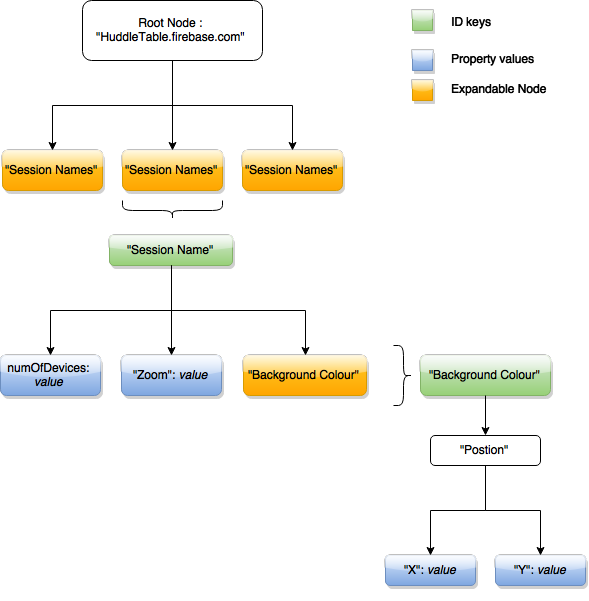
\includegraphics[scale=0.6]{firebase_design}
\caption{My Firebase database design}
\label{firebase_design}
\end{figure}


\subsection{Applications}

\subsubsection{Table App} \label{tableapp}
talk about background color
\subsubsection{Camera App} \label{cameraapp}
talk about session name
\begin{enumerate}
\item problem 
\item how I am going to solve it.
\item What I did
\item evaluation
\end{enumerate}
    